\section{Experiments}
\label{sec:experiments}


\subsection{Robot's Model Training}
\label{subsec:robotmodeltraining}

Before we jumped into training, we make a new dataset which is a merge of NimbRo's Humanoid Robot Pose dataset and Ichiro's dataset.
This dataset contains both single and multiple humanoid robots with type kid-sized, teen-sized, and adult-sized according to Robocup rules.
Most of NimbRo's dataset consists of robots with skin and Ichiro's dataset only consists of robots without skin.
Overall, after merging there are approximately 2.1k images, about 20 percent of the dataset was used for scoring and validating.

There are three models that we try to retrain with the new dataset. Two of them use a bottom-up approach and one uses a top-down approach.
The first one is NimbRo's model, the hyperparameters that are used to train this model followed the description in their paper.
This model is trained using the AdamW optimizer with a learning rate of 10\textsuperscript{-4},
batch size 16, and weight decay of 10\textsuperscript{-4} for the total 200 epochs.
Note that the encoder is initialized by pre-trained ResNet weights on ImageNet.
We also use data augmentation that includes random scaling and random translation during training \citep{amini2021}.
We do not use random horizontal flip and random rotation like NimbRo did because in our case it will make the training result worse.

YOLO-pose is the second model that we retrain.  However, we must convert the format of our newly created dataset from COCO to YOLO.
Differ from COCO format, YOLO format gives keypoint confidence or visibility flag 2 for either visible or occluded keypoint
and if it is outside the field of view, the value is set to zero. However, COCO defines visibility flag as v=0: not labeled, v=1: labeled but not visible, and v=2: labeled and visible. So, we change the definition of
v=1 and v=2 become just v=2 in YOLO format and keep v=0.
Beside keypoint format differences, bounding-box format between them is also different. COCO defines a bounding-box as follow: x (top left), y (top left), width, and height. On the other hand,
bounding-box format in YOLO is: x (center), y (center), width, and height also all of them need to be normalized. Thus, we need to add 1/2 width to x, 1/2 height to y, and normalize them.
The hyperparameters to train YOLO-pose followed the description in their GitHub named \emph{hyp.pose.yaml}.
We use SGD optimizer with a cosine scheduler. The base learning rate is set to 10\textsuperscript{-2}, batch size 16,
and weight decay of 5\textsuperscript{-4} for total 150 epochs. There are also data augmentation like random scale [0.5, 1.5],
random translation [-10, 10], random flip with probability 0.5, mosaic augmentation with probability 1, and various color augmentations.

Lastly, we train Keypoint RCNN using PyTorch. By default, the \emph{AnchorGenerator} class in PyTorch has 3 different sizes (128, 256, 512) and 3 different aspect ratios (0.5, 1.0, 2.0).
We have extended those parameters, \emph{AnchorGenerator} to (32, 64, 128, 256, 512) and \emph{aspect ratios} to (0.25, 0.5, 0.75, 1.0, 2.0, 3.0, 4.0).
In this training, we use SGD optimizer with learning rate 10\textsuperscript{-3}, batch size 3, and weight decay of 5\textsuperscript{-4} for 50 epochs.
For augmentation, we use random rotation, brightness, and contrast

All of the tests were conducted using the Ichiro robot in the \emph{Robot Cerdas} Laboratory with computer specifications as can be seen in Table \ref{tb:computerspecichiro}.
Table \ref{tb:robotmodelcomparison} shows the evaluation metrics results of three models.
NimbRo and RCNN use the Object Keypoint Similarity (OKS) with a per-keypoint constant equal to 0.4 for all keypoints.
Otherwise, YOLO uses slightly different OKS, they extend the idea of IOU loss from box to keypoints. OKS is treated as IOU in case of keypoints \citep{maji2022yolopose}.
It can be seen that RCNN has the highest evaluation metric among the other models.
Moreover, RCNN showed the best detection results as shown in Table \ref{tb:robotmodelcomparisondetectionresults}, followed by NimbRo and YOLO-pose.
Lastly, Nimbro is the most likely to be applied to real-time systems because it has the lowest inference time as shown in Table \ref{tb:inferencerobot}.
However, since our main program uses the web for interaction and during PLAY mode, there is a considerable delay due to transferring two image data from the server to the client.
Hence, we decide to store the images first and do pose comparisons afterwards. Since we are more concerned with a reliable model than a faster model, so the RCNN model is suitable for this.

\begin{table}
\caption{Computer specification on Ichiro robot.}
\centering
    \begin{tabular}{|c|c|}
    \hline
    OS      & Ubuntu 20.04.2 LTS \\
    \hline
    CPU     & Intel i5-10210U (8) @ 4.200GHz \\
    \hline
    GPU     & Intel UHD Graphics  \\
    \hline
    RAM     & 3636 MiB \\
    \hline
    \end{tabular}
    \label{tb:computerspecichiro}
\end{table}

\begin{table*}[h!]
\caption{Robot Model Comparison.}
\centering
    \begin{tabular}{|c|c|c|c|c|c|c|c|c|c|c|} 
    \hline
    \rowcolor{lightgray} \textbf{Model} & \textbf{AP} & \textbf{AP\textsubscript{50}} & \textbf{AP\textsubscript{75}} & \textbf{AP\textsubscript{M}} & \textbf{AP\textsubscript{L}} & \textbf{AR} & \textbf{AR\textsubscript{50}} & \textbf{AR\textsubscript{75}} & \textbf{AR\textsubscript{M}} & \textbf{AR\textsubscript{L}} \\ 
    \hline
    NimbRo         & 0.828       & 0.879                         & 0.840                         & 0.886                        & 0.864                        & 0.836       & 0.884                         & 0.849                         & 0.895                        & 0.872 \\
    \hline
    RCNN           & 0.879       & 0.936                         & 0.904                         & 0.859                        & 0.937                        & 0.925       & 0.973                         & 0.944                         & 0.936                        & 0.955 \\
    \hline
    YOLO           & 0.849       & 0.838                         & -                             & -                            & -                            & 0.814       & -                             & -                             & -                            & - \\
    \hline
    \end{tabular}
    \label{tb:robotmodelcomparison}\\
\end{table*}

\begin{table*}
\caption{Robot Model Comparison Detection Results.}
\centering
    \begin{tabular}{|c|c|c|}
    \hline
    \rowcolor{lightgray}
    \textbf{NimbRo}    & \textbf{RCNN} & \textbf{YOLO-pose}\\
    \hline
    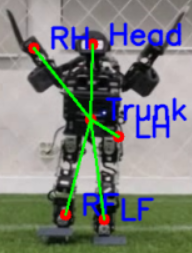
\includegraphics[scale=0.75]{gambar/nimbro-1.png} & 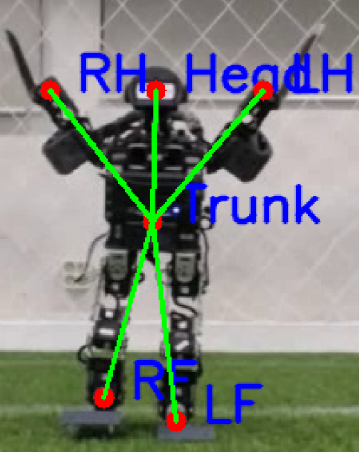
\includegraphics[scale=0.75]{gambar/rcnn-1.png} & 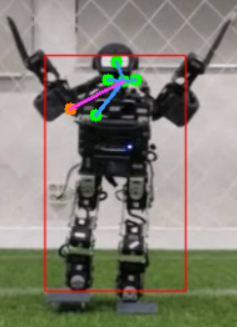
\includegraphics[scale=0.75]{gambar/yolo-1.png} \\
    \hline
    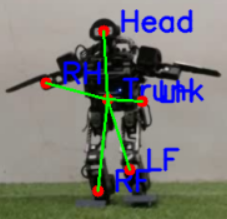
\includegraphics[scale=0.75]{gambar/nimbro-2.png} & 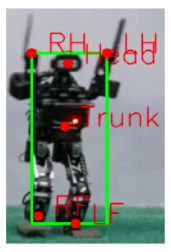
\includegraphics[scale=0.75]{gambar/rcnn-2.png} & 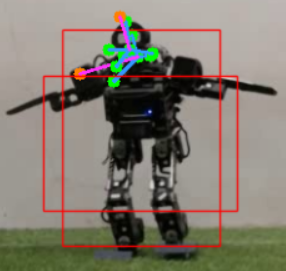
\includegraphics[scale=0.75]{gambar/yolo-2.png} \\
    \hline
    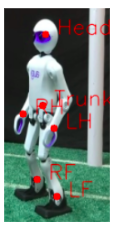
\includegraphics[scale=0.75]{gambar/nimbro-3.png} & 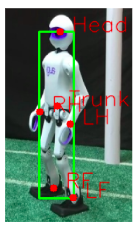
\includegraphics[scale=0.75]{gambar/rcnn-3.png} & 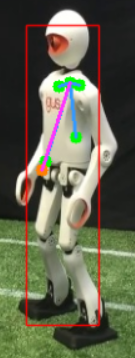
\includegraphics[scale=0.75]{gambar/yolo-3.png} \\
    \hline
    \end{tabular}
    \label{tb:robotmodelcomparisondetectionresults}\\
\end{table*}

\begin{table}
\caption{Inference Time Model Humanoid Robot.}
\centering
    \begin{tabular}{{|c|c|c|}}
    \hline
    \rowcolor{lightgray}
    \textbf{Model}    & \textbf{PyTorch (s)} & \textbf{OpenVINO (s)}\\
    \hline
    NimbRo's Model & 0.4 - 0.5 & 0.15 - 0.2 \\
    \hline
    RCNN Keypoint  & 3.5 - 4.0 & 1.25 \\
    \hline
    YOLO-pose      & 0.7 - 0.75& 0.27 - 0.3 \\
    \hline
    \end{tabular}
    \label{tb:inferencerobot}
\end{table}


\subsection{Human's Model Comparison}
\label{subsec:humanmodelcomparison}

Based on study held by \citet{bazarevsky2020} that compares three different models: BlazePose Lite, BlazePose Full, and OpenPose (body only), they test the models on AR Dataset and Yoga Dataset. As an evaluation metric, they use the Percent of Correct Points with 20\% tolerance (PCK@0.2)
(where assuming the point to be detected correctly if the 2D Euclidian error is smaller than 20\% of the corresponding person's torso size). BlazePose shows slightly worse performance than the OpenPose model on the AR dataset but BlazePose Full outperforms OpenPose on Yoga/Fitness use cases.
Note that, in this study, we use BlazePose Full because by default the value of \emph{model complexity} argument is 1 in the \emph{mediapipe.solutions.pose.Pose} API class. Mediapipe provides 3 BlazePose models: BlazePose Lite, BlazePose Full, and BlazePose Heavy. Pose landmark accuracy as well
as inference latency generally go up with the model complexity.
Since in this study, we just need single-person pose detection, MediaPipe should be the best and also a reliable choice.


\subsection{Comparing the Suitability Between Humanoid Robot Pose and Human Pose}
\label{subsec:comparingsuitability}

The difference in numbers between human keypoints and robot keypoints makes us have to reduce human keypoints in order to make a comparison between them.
Based on the results Subsection \ref{subsec:robotmodeltraining} and \ref{subsec:humanmodelcomparison}, we chose Mediapipe for human and Keypoint RCNN for robot.
Mediapipe provides 33 landmark keypoints for human and Keypoint RCNN only provides 6 keypoints.
Therefore, we need to reduce the human keypoint to 6, such as the head keypoint which is located between the right and left eyes.
The keypoint for the hands and feet is simply to select the wrists and ankles in Mediapipe, where landmark[15] and landmark[16] are wrists, landmark[27] and landmark[28] are ankles.
Lastly, the trunk keypoint is located between the shoulder and hip keypoint.

\begin{figure}[ht]
\centering
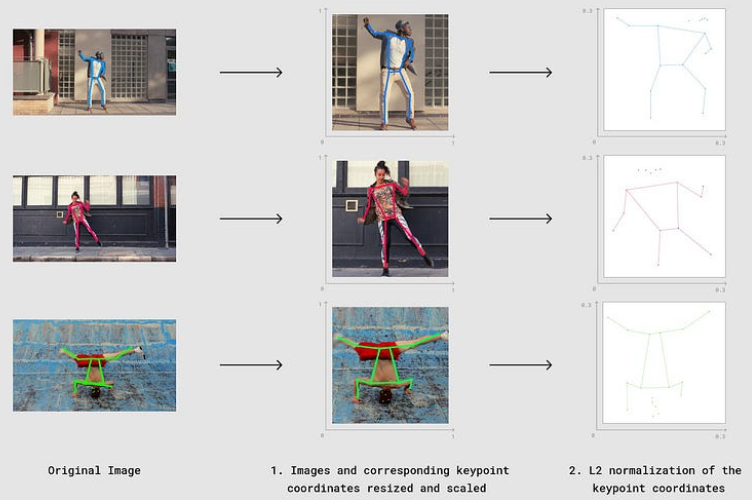
\includegraphics[scale=0.52]{gambar/two-steps.png}
\caption{Steps Taken to Normalize Data.}
\label{fig:steps-to-normalize}
\end{figure}

The next step is defining similarity. When we think about the problem, we see that there are many uncertainties to be addressed. For example, human and humanoid robot can differ in height, body shape, and location within an image: one subject (human or robot) may have been nearby the camera,
while another may have been in the distance. In order to get an accurate outcome, each of these issues must be resolved.
After reducing the keypoints, the model output for both human and robot is the coordinates of 6 keypoints. This information can be used to create a new bounding box that tightly covers the person in the picture. 
This solves the problem of the subject appearing in different parts of the picture.
We further normalized the resulting keypoints coordinates by performing L2 normalization in order to transform it into a unit vector.
This means we are ignoring the size of the picture, but keeping in account the direction of the vector, created by the pose inside of that image.
The two steps described before can be thought of visually as shown in Figure \ref{fig:steps-to-normalize}.

Now that we have standardized the pose vectors, it is time to choose a similarity measure. We chose cosine similarity for this particular instance, mainly because we are working with vectors
and performing a few calculations detailed below to arrive at a Euclidean distance that can be interpreted as a cosine distance.
The formula shown in Equation \ref{eq:euclideandistance}.
In that formula, Fxy and Gxy are two pose vectors to be compared after L2 normalization. Moreover, Fxy and Gxy contain only x and y positions for each of the 6 keypoints, it does not include confidence scores.

\begin{equation}
    \label{eq:cosinesimilarity}
    cosineSimilarity(x,y) = \frac{x \cdot y}{|x||y|}
\end{equation}
  
\begin{equation}
    \label{eq:euclideandistance}
    D(F_{xy}, G_{xy}) = \sqrt{2 * (1 - cosineSimilarity(F_{xy}, G_{xy}))}
\end{equation}

By using the method before, we get the result from comparing the human pose and robot pose in percentage terms.
We can see the two figures below, in Figure \ref{fig:comparingb} humans make movement that are more like robot than in Figure \ref{fig:comparinga}.
Therefore, the comparison result of Figure \ref{fig:comparingb} is higher at 91\% than Figure \ref{fig:comparinga} with just 79\%.

\begin{figure*}
\centering
\subfloat[Human Image A]{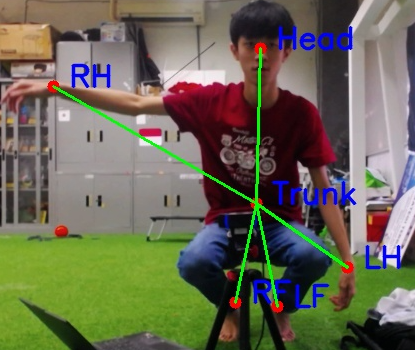
\includegraphics[width=.35\textwidth]{gambar/human_10_result.jpg}
    \label{fig:humanimagea}}
\hfil
\subfloat[Robot Image A]{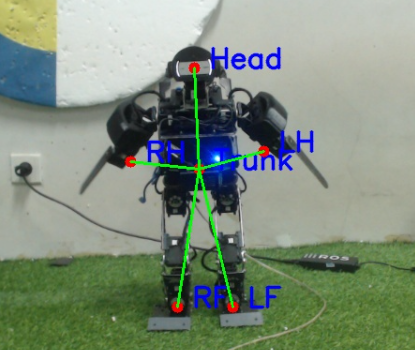
\includegraphics[width=.35\textwidth]{gambar/robot_6_result.jpg}
    \label{fig:robotimagea}}
\caption{Comparing Humanoid Robot Pose and Human Pose.}
\label{fig:comparinga}
\end{figure*}

\begin{figure*}
\centering
\subfloat[Human Image B]{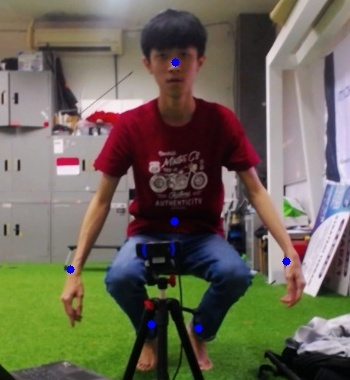
\includegraphics[width=.35\textwidth]{gambar/human_6_result.jpg}
    \label{fig:humanimageb}}
\hfil
\subfloat[Robot Image B]{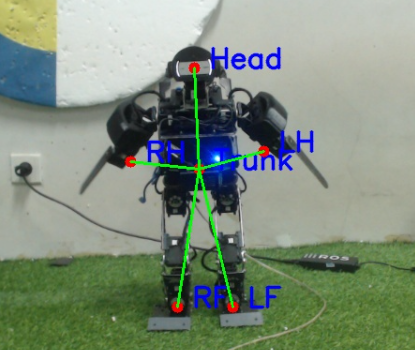
\includegraphics[width=.35\textwidth]{gambar/robot_6_result.jpg}
    \label{fig:robotimageb}}
\caption{Comparing Humanoid Robot Pose and Human Pose.}
\label{fig:comparingb}
\end{figure*}